\documentclass[11pt,a4paper,onecolumn]{article}
\usepackage[T1]{fontenc}
\usepackage[utf8]{inputenc}
\usepackage{lmodern}
\usepackage[margin=23mm]{geometry}
\usepackage{microtype}
\usepackage{amsmath,amssymb}
\usepackage{graphicx}
\usepackage{xcolor}
\usepackage{array,booktabs,tabularx,longtable}
\usepackage{caption,subcaption}
\usepackage{enumitem}
\usepackage{placeins}
\usepackage{tikz,pgfplots}
\usetikzlibrary{arrows.meta,positioning,calc}
\pgfplotsset{compat=1.17}
\usepackage[hidelinks]{hyperref}
\usepackage{url}
\definecolor{ink}{HTML}{203447}
\definecolor{teal}{HTML}{227C80}
\definecolor{softgray}{HTML}{EDF1F4}
\definecolor{warm}{HTML}{B56B42}
\captionsetup{font=small,labelfont=bf,labelsep=period}
\setlist[itemize]{leftmargin=1.5em,itemsep=3pt,topsep=4pt}
\setlist[enumerate]{leftmargin=1.8em,itemsep=3pt,topsep=4pt}
\setlength{\parskip}{5pt plus 1pt}
\setlength{\parindent}{0pt}
\setlength{\tabcolsep}{4pt}
\renewcommand{\arraystretch}{1.17}
\renewcommand{\topfraction}{0.90}
\renewcommand{\textfraction}{0.08}
\renewcommand{\floatpagefraction}{0.75}
\setlength{\emergencystretch}{2em}
\raggedbottom
\newcolumntype{L}[1]{>{\raggedright\arraybackslash}p{#1}}
\newcolumntype{Y}{>{\raggedright\arraybackslash}X}
\newcommand{\artifact}[1]{\nolinkurl{#1}}
\newcommand{\na}{\textemdash}
\pgfplotsset{every axis/.append style={label style={font=\small},tick label style={font=\small},legend style={font=\small,draw=none},axis line style={black!55},grid style={black!12},major tick length=2pt}}

\newsavebox{\methodopeningcheck}
\begin{document}
\setcounter{section}{2}
\begin{lrbox}{\methodopeningcheck}
\begin{minipage}{\linewidth}
\section{Methodology}
\label{sec:methodology}

GRASP connects seven modules around a shared filing record. Figure~\ref{fig:architecture} gives the workflow overview, using the same titles as the following subsections. Filing acquisition provides the common data source, the training branch produces the classifier, and three analytical branches supply the service layer. The arrows highlight the main routes; the module descriptions specify additional database access and shared calculations. In particular, the Transparency Score uses filed-concept coverage, evidence-pattern presence, vagueness flags, and a fixed SDG mapping. Principle probabilities and claim--figure flags remain separate report outputs.

\par\medskip
{\centering
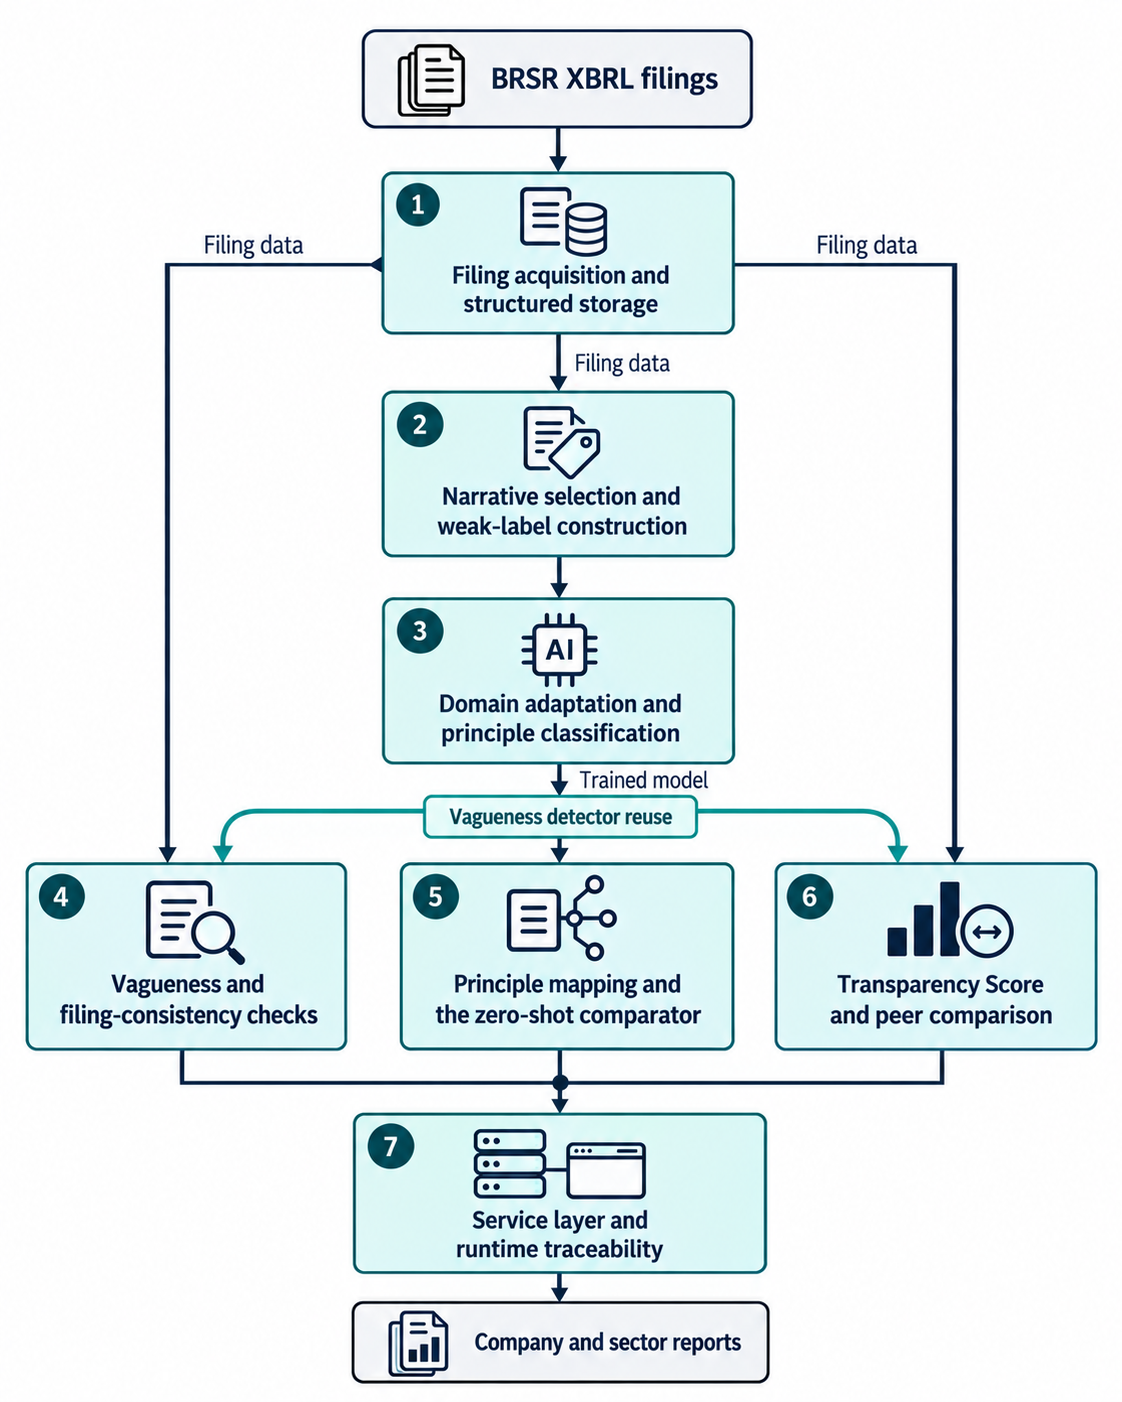
\includegraphics[width=0.98\linewidth,height=0.62\textheight,keepaspectratio]{../figures/grasp_pipeline.png}
\captionof{figure}{GRASP workflow from BRSR filings to company and sector reports. Module titles match the methodology subsections. The training branch supplies the recovered classifier; three analytical branches feed the service layer. Arrows show the main routes. Principle mapping also reads filing narratives, and scoring computes the vagueness signal used for Clarity. Numerical and assurance checks remain review heuristics without a complete validation estimate.}
\label{fig:architecture}
\par}

\end{minipage}
\end{lrbox}
\ifdim\dimexpr\ht\methodopeningcheck+\dp\methodopeningcheck\relax>\textheight
\PackageError{GRASP-layout}{Methodology opening exceeds one page}{Reduce the diagram height before publication.}
\fi
\ifdim\wd\methodopeningcheck>\textwidth
\PackageError{GRASP-layout}{Methodology opening exceeds the text width}{Reduce the block width before publication.}
\fi
\noindent\usebox{\methodopeningcheck}
\end{document}
